\documentclass{article}

% Packages for setting up page margins
\usepackage[margin=1in]{geometry}

\usepackage{graphicx, setspace, amsmath, mathtools, amssymb, url}
\setlength{\parskip}{2mm}
\graphicspath{ {./images/} }

% Title
\title{CS535 Design and Analysis of Algorithms - Assignment 2}
\author{Batkhishig Dulamsurankhor - A20543498}
\date{\today} % Use \date{} for no date

\begin{document}

\maketitle

\section*{Problem 1}
\textbf{Solution:}

\section*{Problem 2}
\textbf{Solution:}

In Fibonacci heaps, we do not have One Rank Rule like in Binomial heap. However, if we were to minimize the number of nodes in the
heap, we must have the higher rank tree to be built with the minimum number of nodes for the lower rank tree. That way we can end up with the fewest possible nodes.
Let's say we have $k$ number of trees, meaning the rank of the biggest tree is $k$. Let's start the recurrence with the first few trees.

\begin{figure}[h]
  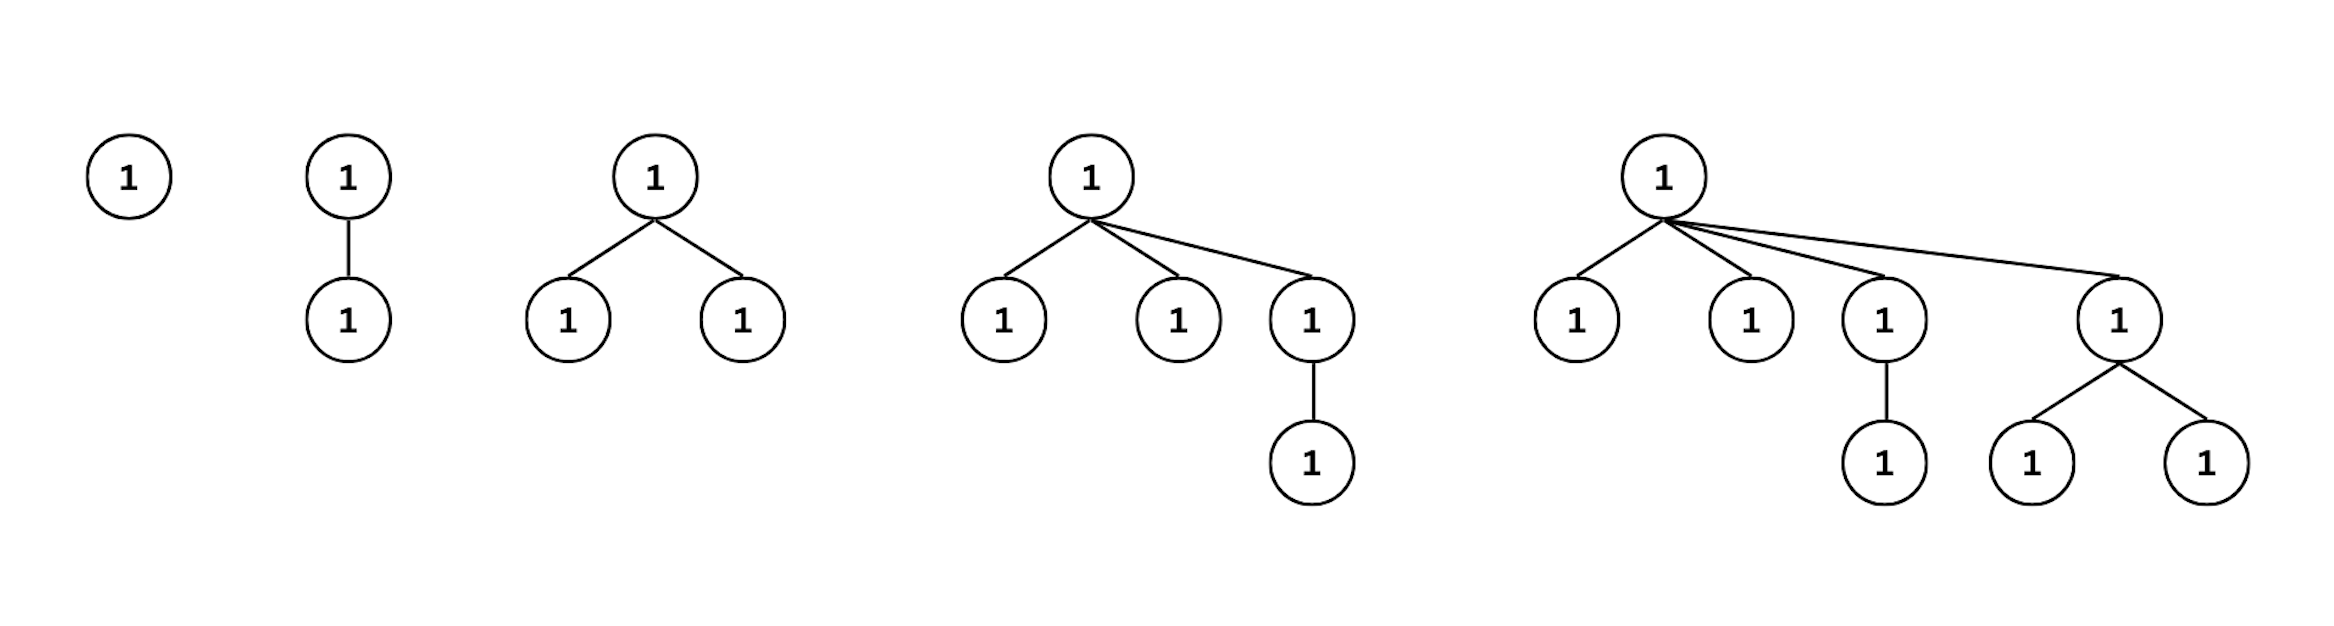
\includegraphics[width=\textwidth]{image1.png}
  \caption{Disclaimer: Each tree has a valid heap structure (not 1s)}
  \centering
\end{figure}

If we look closely, $r=2$ tree is made up of $r=0$ and $r=1$ trees, $r=3$ tree is made up of $r=2$ and $r=1$ trees and on and on.
In other words, the number of nodes at $N_k=N_{k-1}+N_{k-2}$, which is a Fibonacci sequence.

So the minimum number of nodes in the Fibonacci heaps will become the following according to the Fibonacci sequence expression\cite{wiki}:

$N_k=((1+\sqrt(5))^k-(1-\sqrt(5))^k)/\sqrt(5).$

\section*{Problem 3}
\textbf{Solution:}

As we have discussed on the previous problem, we need to be left with only one tree that is made up with the previous two trees.
$N_k=N_{k-1}+N_{k-2}$. The tree is left with subtrees of all the previous ranks that are marked, decrease key has been executed
once for each of them.

\section*{Problem 4}
\textbf{Solution:}

Insertion bound stays the same for allowing $k$ children to be deleted before deleting a node.
Since insertion doesn't involve cutting a node, the amortized cost is still $O(1)$.

Allowing $k$ subtrees to be cut before cutting the node makes the algorithm lose its Fibonacci property, unless $k=1$.
For decrease key, the time complexity is still amortized $O(1)$. Because, decreasing $n$ number of nodes will now result in maximum $n+n/k$
number of trees which is less than Fibonacci heap's $n+n$ when $k>1$.

For delete min, let's say the heap has the minimum value in a maximum rank tree $r$. When the root is removed, each of the children becomes a new root.
It takes $O(r)=O(logn)$ to execute this step. Next, We have to merge the trees with the same rank.
However, we can potentially have many trees with the same rank depending on $k$. That makes the merge operation costly compared to Fibonacci's heap.
The cost for merging step is $O(logn+f(k))$, here $f(k)$ is a function depends on the variable $k$ that represents number of trees before merging.
And finally, we have update the minimum pointer which takes $O(logn)$. Overall, the running complexity is bounded by $O(logn+f(k))$.

The recurrence has been solved in question no2.

\section*{Problem 5}
\textbf{Solution:}

\begin{thebibliography}{9}

\bibitem{wiki}
Bucket queue, \emph{Wikipedia}, \url{https://en.wikipedia.org/wiki/Fibonacci_sequence#Relation_to_the_golden_ratio}

\bibitem{algo}
Skiena, Steven S. (1998), \emph{The Algorithm Design Manual}, Springer, p. 181.

\end{thebibliography}


\end{document}